\section{Life Support Systems Integration and Equivalent System Mass Analysis}
\label{sec:esm_analysis}

\subsection{Equivalent System Mass Accounting Framework}
\label{subsec:esm_framework}

To evaluate the flight viability of life-support hardware, space systems architects employ the Equivalent System Mass ($\mathrm{ESM}$) metric, formalized in NASA's \textit{Advanced Life Support Baseline Values and Assumptions Document} (BVAD)\cite{hanford2004advanced,hanford2006baseline}. $\mathrm{ESM}$ converts physical mass, pressurized volume, operational power, thermal rejection, and crew maintenance labor into a single standardized mass figure ($\mathrm{kg}$)\cite{hanford2004advanced,bilardo2024equivalent}:
\begin{equation}
    \mathrm{ESM} = M + \left(V \cdot C_V\right) + \left(P \cdot C_P\right) + \left(C \cdot C_C\right) + \left(T \cdot C_T\right)
    \label{eq:esm_formulation}
\end{equation}
where $M$ is hardware and consumable mass ($\mathrm{kg}$), $V$ is pressurized habitat volume ($\mathrm{m}^3$), $P$ is operational electrical power demand ($\mathrm{kWe}$), $C$ is thermal cooling rejection load ($\mathrm{kWth}$), and $T$ is routine crew maintenance time ($\mathrm{crew\text{-}hours/year}$)\cite{hanford2004advanced,hanford2006baseline}. The infrastructure equivalency factors---$C_V$ ($\mathrm{kg/m}^3$), $C_P$ ($\mathrm{kg/kWe}$), $C_C$ ($\mathrm{kg/kWth}$), and $C_T$ ($\mathrm{kg/crew\text{-}hour}$)---quantify the launch mass required to supply an incremental unit of that resource on the lunar surface\cite{hanford2004advanced,bilardo2024equivalent}.

On the Moon, these equivalency factors depend heavily on the outpost power architecture\cite{anderson2021lunar,vos2020internal}. For photovoltaic arrays paired with regenerative fuel cells or lithium-ion batteries ($200\,\mathrm{Wh/kg}$), the 14-day lunar night drives $C_P$ to $\sim 237\,\mathrm{kg/kWe}$\cite{vos2020internal,colozza2020power}. Surface fission reactors reduce $C_P$ to approximately $54\text{--}100\,\mathrm{kg/kWe}$\cite{colozza2020power}. Meanwhile, radiating waste heat into a lunar vacuum remains challenging, maintaining high thermal infrastructure factors ($C_C \approx 85\text{--}145\,\mathrm{kg/kWth}$)\cite{vos2020internal,ewert2020thermal}. Consequently, agricultural systems with high recurring consumable resupply or extensive crew maintenance quickly incur severe lifecycle mass penalties\cite{ming1989lunar,hanford2004advanced,ewert2020thermal}.

\subsection{Comparative Lifecycle Assessment: Direct Agriculture versus Sintered Infrastructure}
\label{subsec:comparative_lca}

Comparing direct regolith agriculture against sintered ceramic bio-infrastructure reveals fundamental trade-offs between initial deployment mass and long-term operational sustainability\cite{ming1989lunar,hanford2004advanced} (Table~\ref{tab:esm_comparison} and Figures~\ref{fig:esm_lifecycle}--\ref{fig:mission_economics}):

\subsubsection{Water Recovery Efficiency}
Water recycling is a dominant driver of lifecycle $\mathrm{ESM}$\cite{hanford2004advanced,bilardo2024equivalent}. In direct regolith cultivation, water loop closure is severely compromised\cite{ming1989lunar}. Due to the immense specific surface area of sub-micrometer dust and tortuous pore networks, $15\text{--}20\%$ of applied irrigation water becomes immobilized in fine micropores at matric potentials below the permanent wilting point ($\psi_m < -1.5\,\mathrm{MPa}$)\cite{paul2022plants,ming1989lunar,hendrix2024reactivity}. This water cannot be extracted by plant roots and resists passive evaporation into habitat dehumidification systems\cite{ming1989lunar,hendrix2024reactivity}. Consequently, direct regolith farming achieves only $78\text{--}82\%$ water recovery efficiency, requiring hundreds of kilograms of annual makeup water resupplied from Earth or energy-intensive polar ice extraction\cite{ming1989lunar,anderson2021lunar}. In contrast, sintered ceramics feature open, interconnected pore channels that allow both root uptake and negative-pressure recovery\cite{ming1989lunar}. Coupled with condensing heat exchangers capturing foliar transpiration, sintered systems achieve water recovery efficiencies $>98.5\%$, drastically lowering ongoing logistics mass\cite{ming1989lunar,wheeler2023space}.

\subsubsection{Chemical Nutrient Solution Stability}
Direct cultivation in raw regolith destabilizes hydroponic chemistry\cite{ming1989lunar,schoonen2020hydroxyl}. Exposure to aqueous solutions ($\mathrm{pH}\;5.5\text{--}6.5$) induces uncontrolled dissolution of plagioclase, olivines, and pyroxenes, releasing excess divalent and alkali cations ($\mathrm{Ca}^{2+}, \mathrm{Mg}^{2+}, \mathrm{Na}^+$) that trigger rapid alkaline spikes ($\mathrm{pH}\;9.0\text{--}11.0$)\cite{ming1989lunar,hendrix2024reactivity,schoonen2020hydroxyl}. This alkaline environment precipitates essential orthophosphate ions ($\mathrm{PO}_4^{3-}$) as insoluble calcium phosphates, while iron, zinc, and manganese precipitate as insoluble hydroxides\cite{ming1989lunar,atkin2024bioremediation,wamelink2024struvite}. Maintaining plant viability requires continuous buffering with concentrated nitric ($\mathrm{HNO}_3$) and sulfuric ($\mathrm{H}_2\mathrm{SO}_4$) acids and synthetic chelating agents (EDTA/EDDHA), consuming $\sim 145\,\mathrm{kg/year}$ of chemical consumables for a nominal 6-person habitat\cite{ming1989lunar,atkin2024bioremediation,lytvynenko2021lunar}. Conversely, regolith sintered above $1050^\circ\mathrm{C}$ forms a vitrified aluminosilicate ceramic that resists aqueous dissolution, providing hydrothermal stability across multi-year operational regimes with stable $\mathrm{pH}$ ($5.8\text{--}6.2$) and minimal buffer resupply ($<8\,\mathrm{kg/year}$)\cite{ming1989lunar}.

\subsubsection{Habitat Dust Mitigation and Crew Maintenance}
Direct regolith agriculture necessitates excavating, transporting, and managing large inventories of abrasive dust inside or adjacent to pressurized modules\cite{paul2022plants,ming1989lunar}. Fugitive airborne dust erodes environmental control and life support system (ECLSS) mechanical seals, fouls air filters, and presents toxicological risks to crew respiratory health\cite{paul2022plants,ming1989lunar,hendrix2024reactivity,wallace2022assessment}. Sintered bio-infrastructure locks loose particles into monolithic ceramic components, eliminating particulate hazards from the habitat atmospheric loop\cite{ming1989lunar}.

\subsubsection{ESM Breakeven Horizon}
Direct regolith cultivation exhibits a lower initial launch mass ($\sim 420\,\mathrm{kg}$ for containment bins and basic tools for a 6-crew module)\cite{paul2022plants,ming1989lunar}. However, its steep recurring consumables slope---driven by water loss, acid buffers, and crew labor---causes cumulative $\mathrm{ESM}$ to escalate rapidly\cite{ming1989lunar,hanford2004advanced,fackrell2024mechanical}. Sintered bio-infrastructure requires a higher upfront launch investment ($\sim 1850\,\mathrm{kg}$ for an automated microwave/solar sintering manufacturing plant)\cite{ming1989lunar,meek1993mechanical}. Systems-level parametric modeling demonstrates that cumulative $\mathrm{ESM}$ curves cross within $18\text{--}22$ months under conservative power assumptions (and as early as $9\text{--}15$ months under surface nuclear power)\cite{ming1989lunar,chinnannan2025spirulina,metzger2023cost}. For mission durations exceeding two years, sintered ceramics yield compounding mass savings, establishing them as the superior edaphic strategy for permanent lunar settlements.

\subsubsection{Operational Phase-In and ESM Breakeven Timeline}
The operational transition from outpost landing to net-positive logistics returns is tracked in the 60-month ISRU manufacturing and deployment Gantt schedule (Figure~\ref{fig:isru_esm_gantt}) and rendered in photorealistic 3D architectural phasing on the Shackleton Crater rim (Figure~\ref{fig:moonbase_3d_phases}):
\begin{itemize}
    \item \textbf{Phase I: Logistics and Beneficiation (Months 0--6, Fig.~\ref{fig:moonbase_3d_phases}a):} Touchdown of cargo landers delivers the $1850\,\mathrm{kg}$ sintering facility and surface power systems (e.g., $40\,\mathrm{kWe}$ Kilopower FSP). Tele-operated excavation rovers extract raw lunar regolith, executing magnetic separation to remove native $\mathrm{npFe}^0$ spherules and sieving feedstock to $<100\,\mu\mathrm{m}$ to ensure uniform dielectric coupling.
    \item \textbf{Phase II: Serial Sintering Manufacturing (Months 3--15, Fig.~\ref{fig:moonbase_3d_phases}b):} The automated microwave sintering plant conducts vacuum thermal consolidation under strict thermal-stress cooling control ($<15^\circ\mathrm{C/min}$). Modular porous ceramic trays and fluidic distribution manifolds are produced and given a hydrothermal passivation rinse, alongside sintered regolith blast berms and landing pads, building the complete substrate inventory for a 6-person habitat within 12 months.
    \item \textbf{Phase III: Canopy Phasing and ESM Breakeven (Months 12--24, Fig.~\ref{fig:moonbase_3d_phases}c):} Sintered trays are mounted into vertical habitat growth racks, plumbed into closed nutrient loops, and seeded under PAR LED grow lighting within pressurized Artemis inflatable/rigid modules and translucent geodesic greenhouse domes. By Month 18.5, cumulative mass savings from avoided water resupply ($>98.5\%$ recovery vs. $80\%$ in raw regolith) and chemical buffer elimination ($<8\,\mathrm{kg/year}$ vs. $145\,\mathrm{kg/year}$) surpass the initial $1850\,\mathrm{kg}$ launch penalty of the manufacturing plant.
    \item \textbf{Phase IV: Compounding Multi-Year Advantage (Months 20--60+, Fig.~\ref{fig:moonbase_3d_phases}d):} Beyond Month 20, the facility enters steady-state autonomous production. Powered by cyclic $500^\circ\mathrm{C}$ pyrolytic substrate regeneration and decoupled microbial bioweathering, the system requires near-zero media resupply. By Month 60, net launch mass savings exceed $8,000\,\mathrm{kg}$ (avoiding $>\$40\mathrm{M}$ in launch resupply costs), providing an overwhelming empirical justification for ISRU-derived ceramics.
\end{itemize}

\begin{figure}[t!]
    \centering
    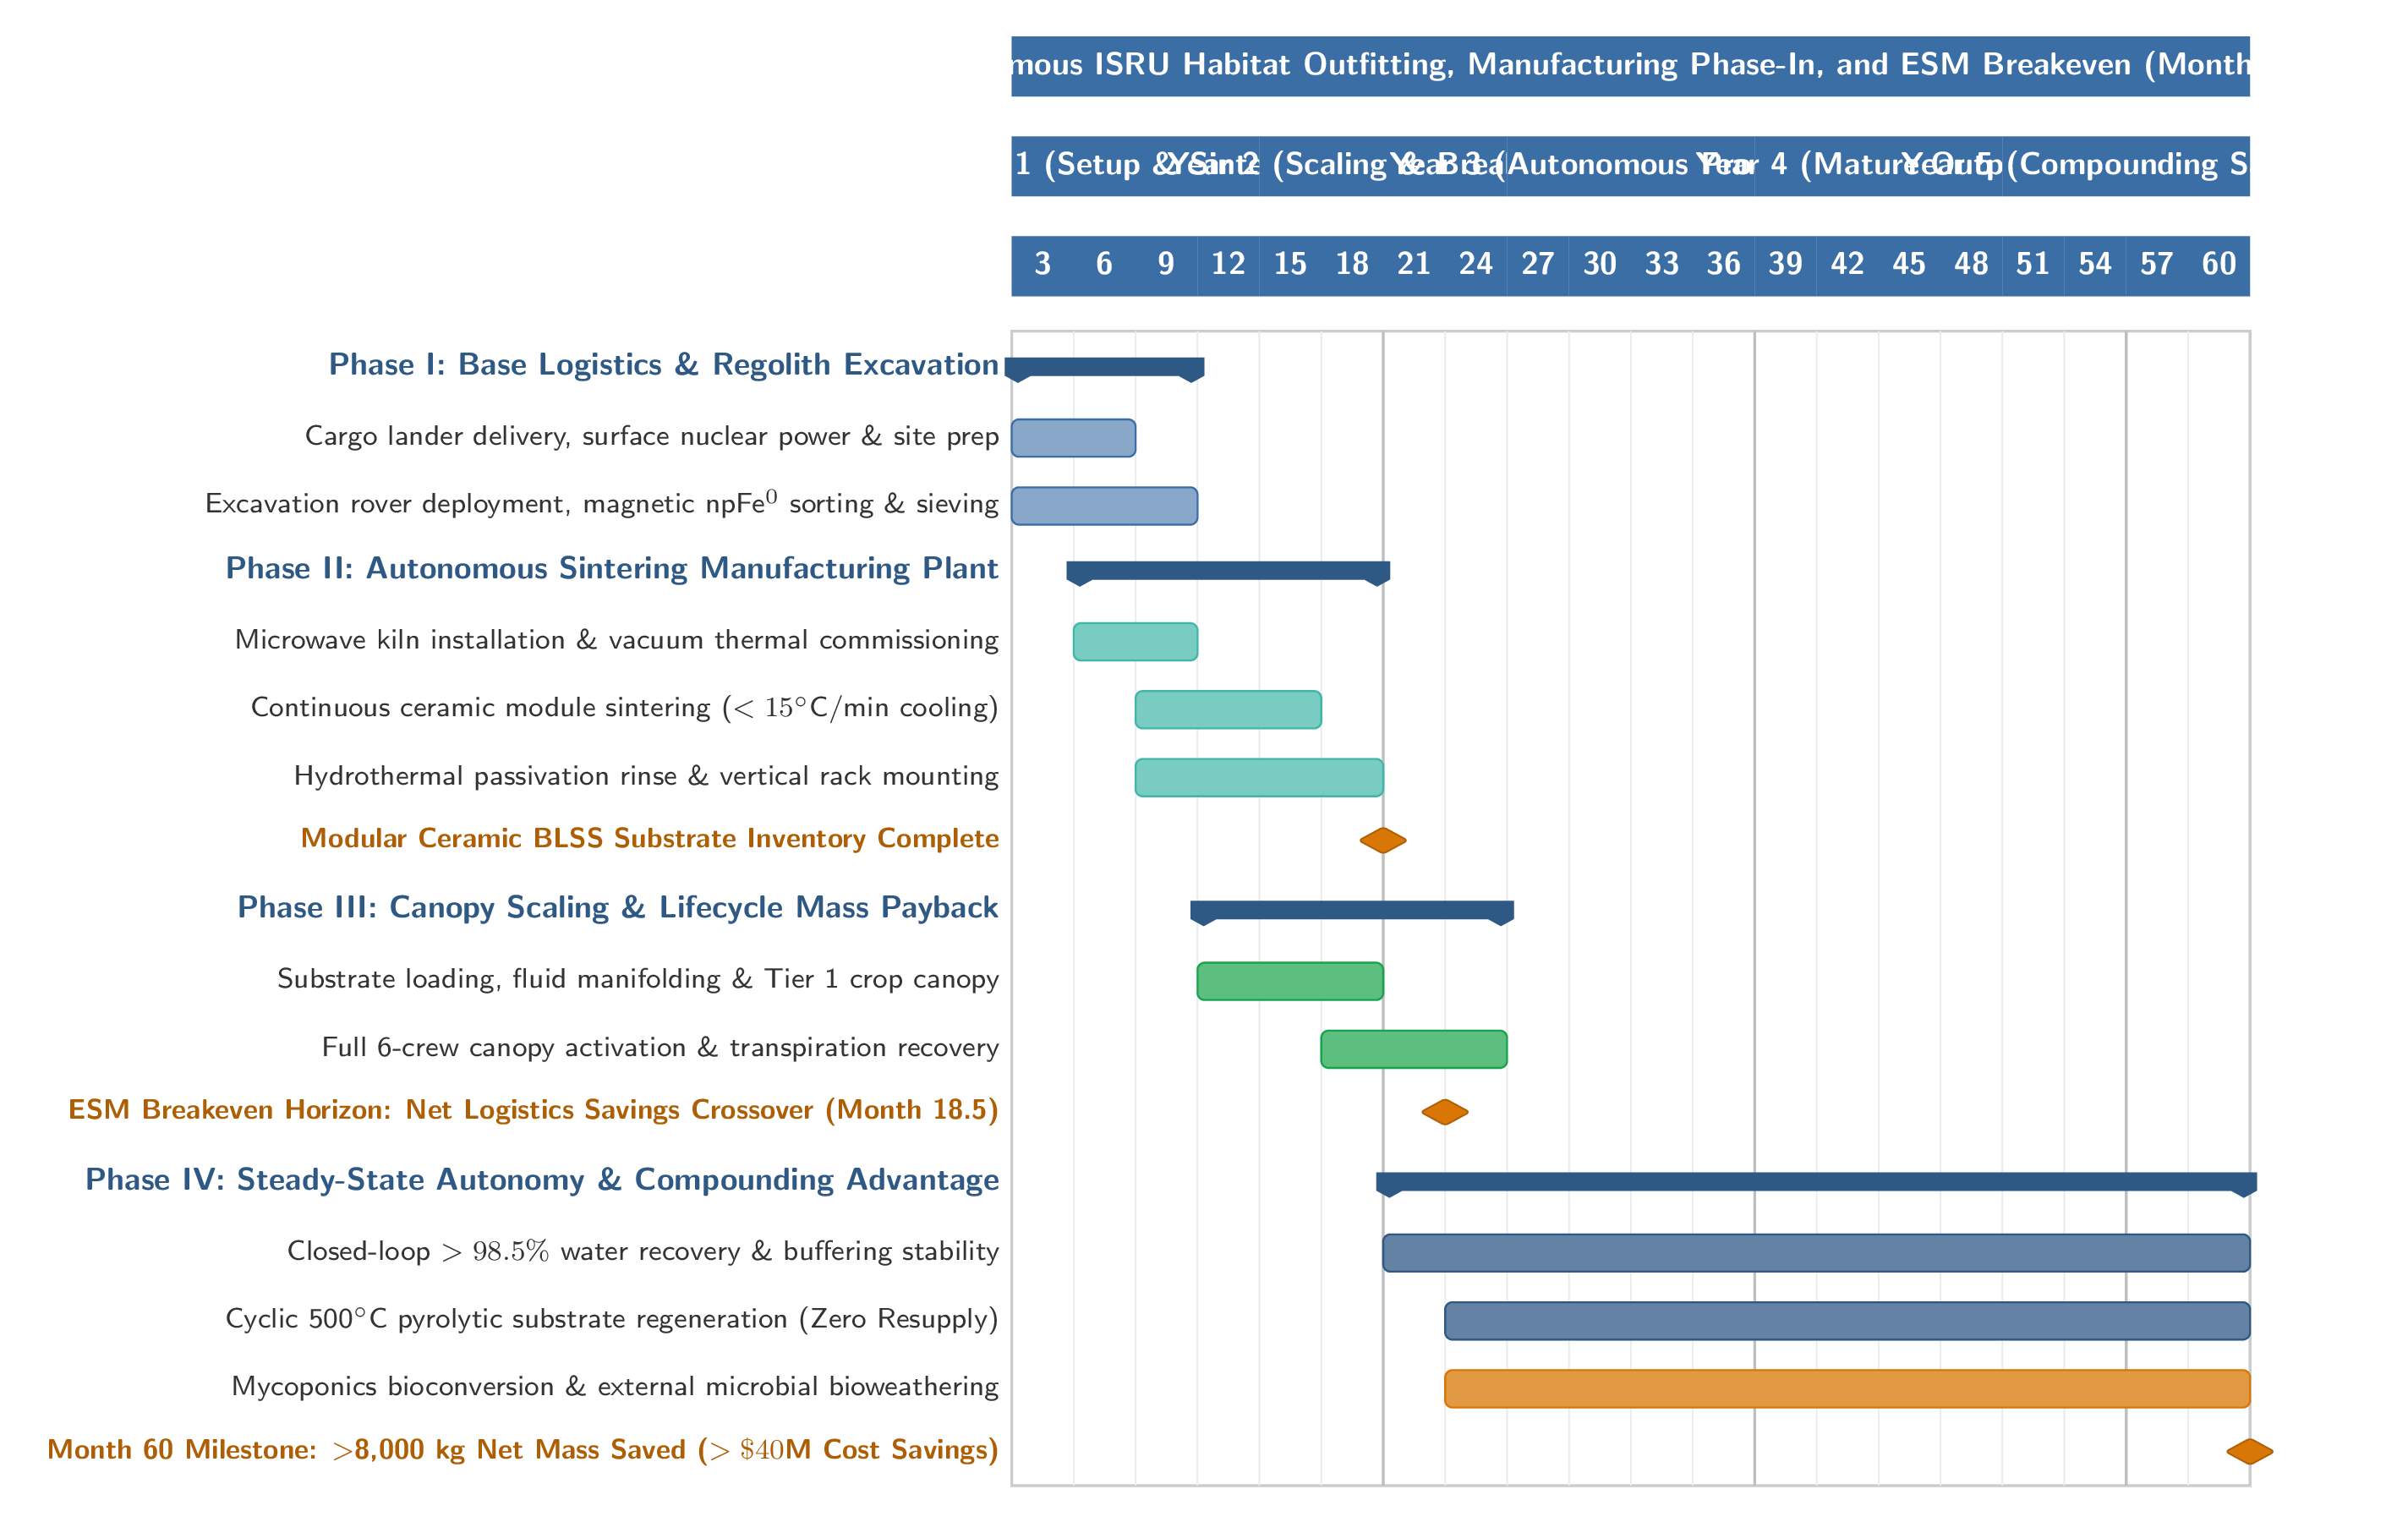
\includegraphics[width=\textwidth]{figures/fig9_isru_esm_gantt.png}
    \caption{\textbf{Autonomous ISRU habitat outfitting, manufacturing phase-in, and Equivalent System Mass (ESM) breakeven timeline.} Phased progression over a 60-month lunar surface mission: Phase I logistics \& excavation (Months 0--6); Phase II automated sintering manufacturing plant operations producing ceramic modular trays (Months 3--15); Phase III canopy scaling and the critical ESM breakeven horizon at Month 18.5, where cumulative logistics savings surpass the $1850\,\mathrm{kg}$ sintering plant launch investment; and Phase IV steady-state autonomous operations achieving compounding savings ($>8,000\,\mathrm{kg}$ net mass and $>\$40\mathrm{M}$ resupply avoidance by Month 60 for a 6-person crew).}
    \label{fig:isru_esm_gantt}
\end{figure}

\begin{figure}[p!]
    \centering
    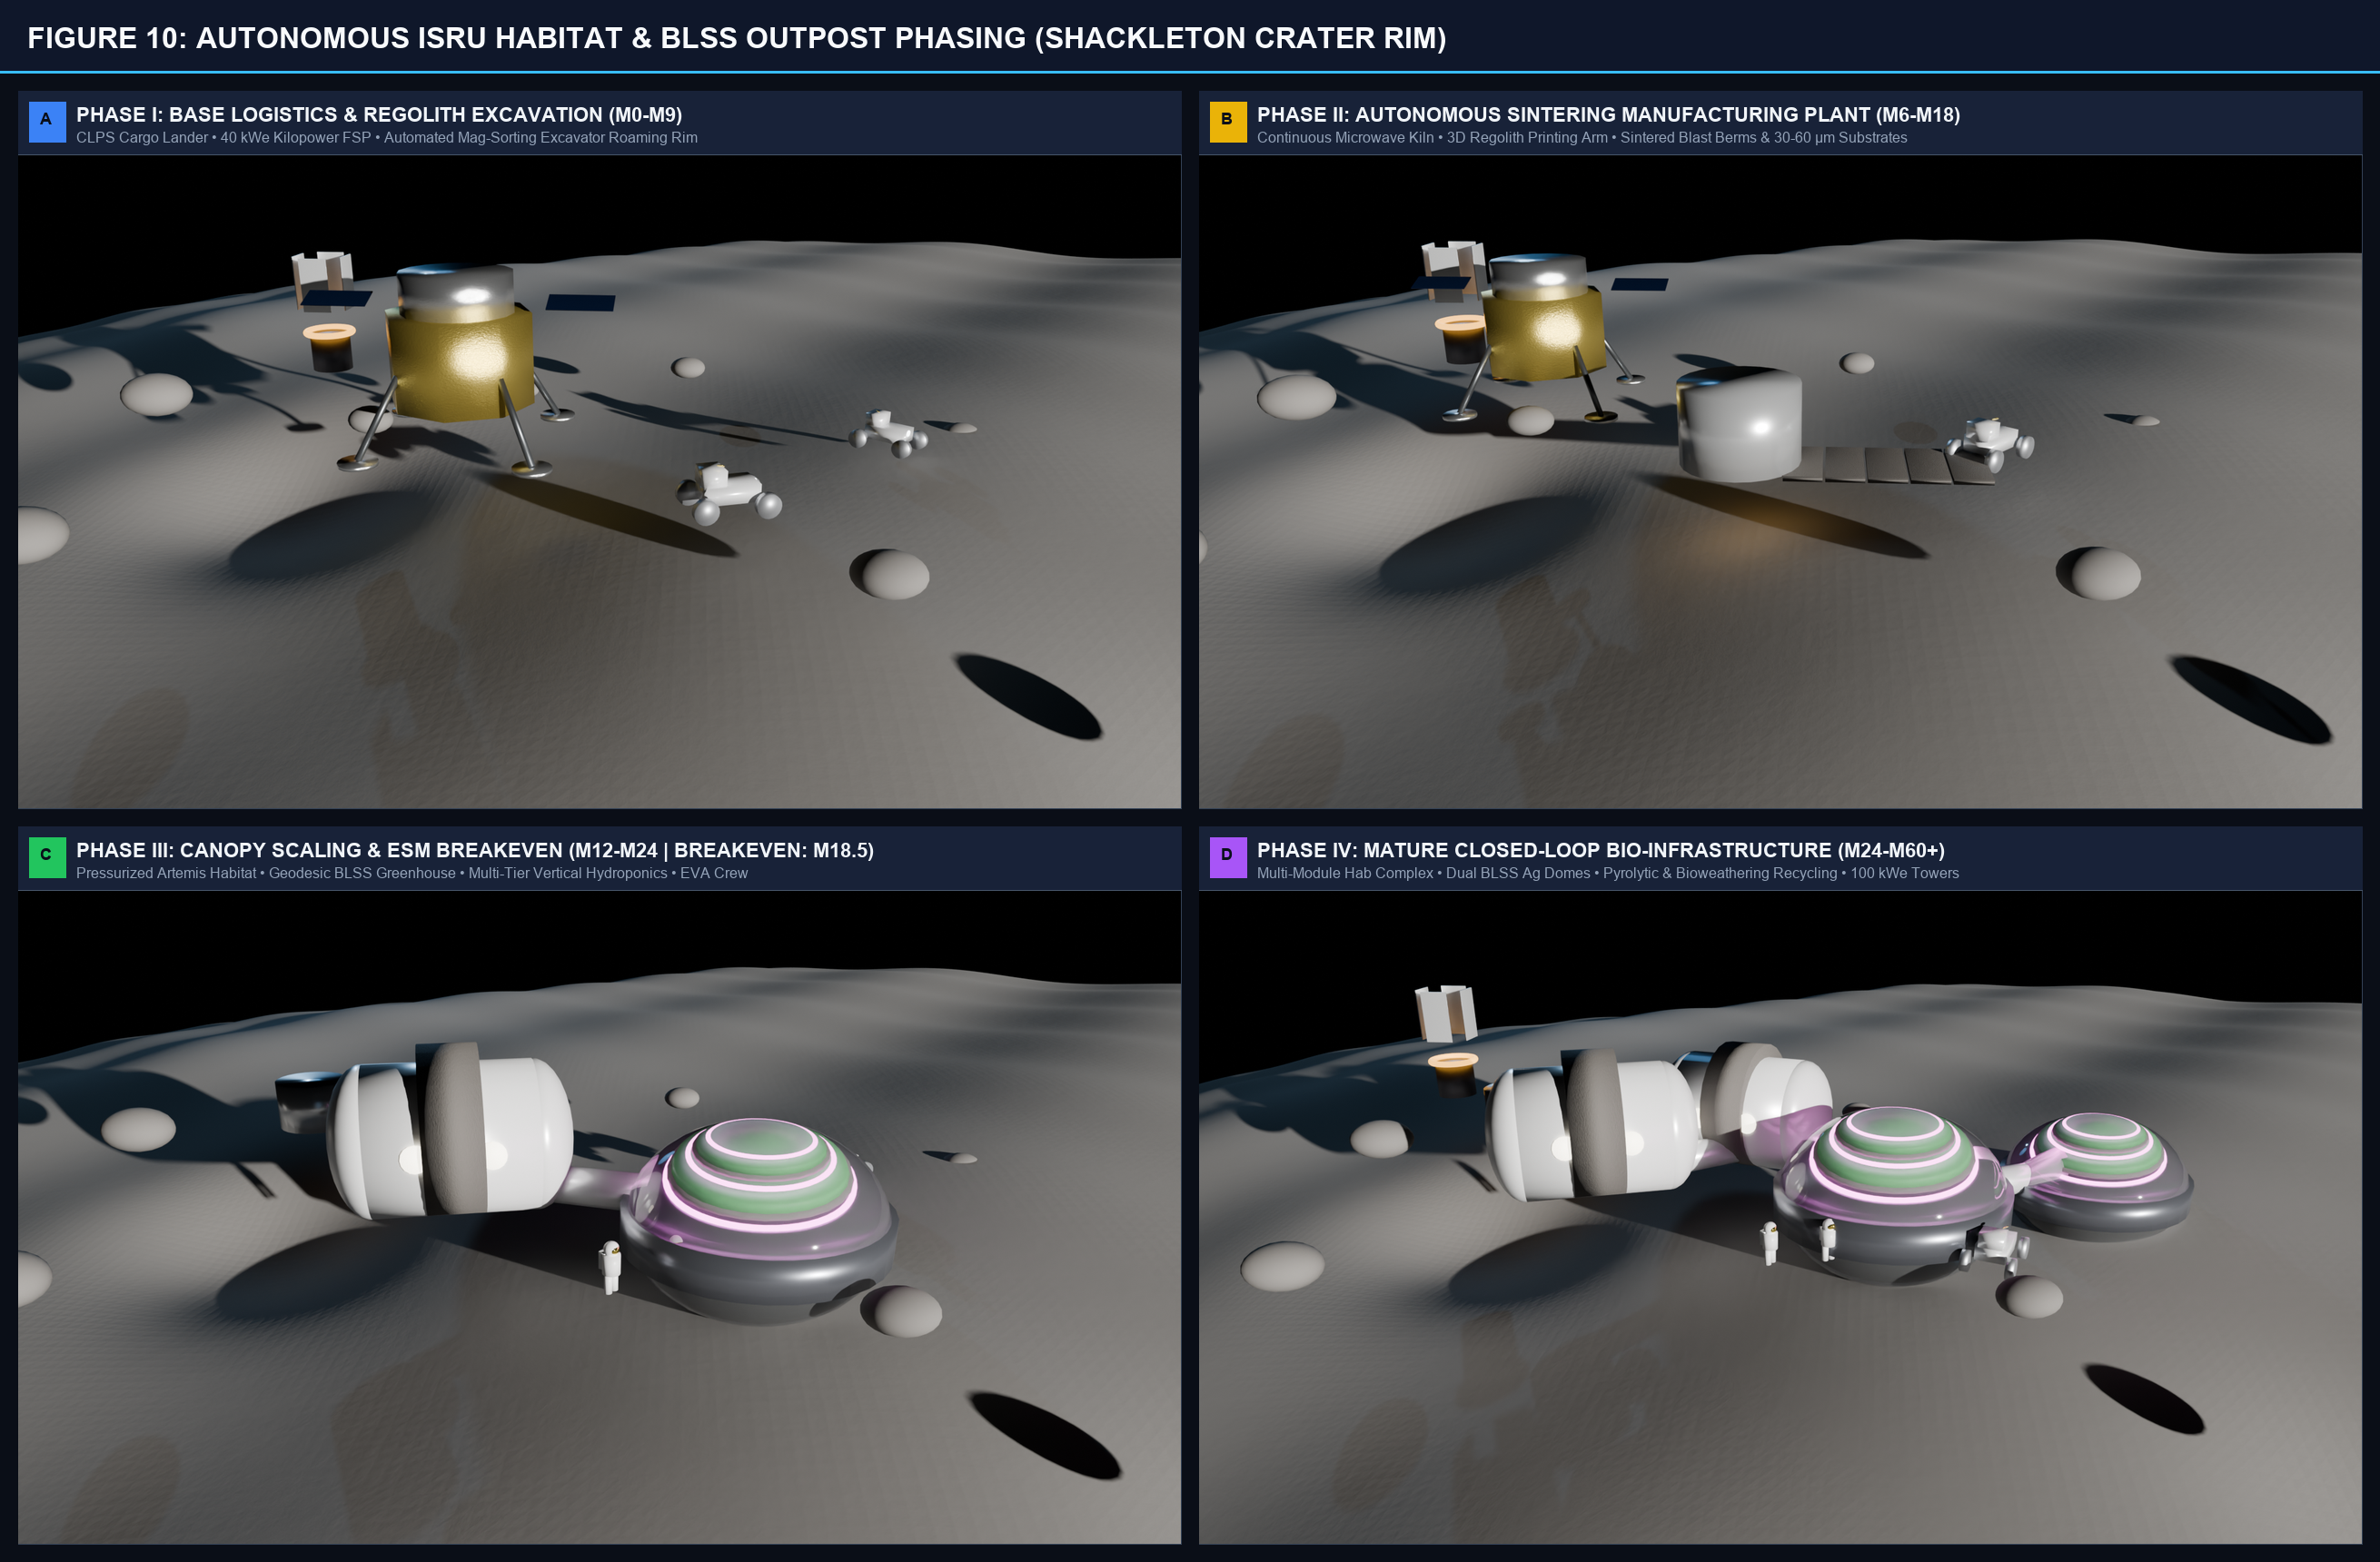
\includegraphics[width=\textwidth]{figures/fig10_moonbase_phases_montage.png}
    \caption{\textbf{Photorealistic 3D architectural progression of autonomous ISRU habitat manufacturing and BLSS bio-infrastructure phasing on the Shackleton Crater rim.} (\textbf{a}) \textbf{Phase I: Base Logistics \& Regolith Excavation (M0--M9):} Commercial Lunar Payload Services (CLPS) cargo lander delivery, deployment of a $40\,\mathrm{kWe}$ Kilopower nuclear fission surface power unit, and automated excavation rovers with high-gradient magnetic beneficiation to remove native $\mathrm{npFe}^0$. (\textbf{b}) \textbf{Phase II: Autonomous Sintering Manufacturing Plant (M6--M18):} Continuous microwave sintering kiln and robotic 3D printing arm producing $30\text{--}60\,\mu\mathrm{m}$ pore-throat ceramic hydroponic substrate blocks, sintered dust-shield perimeter berms, and interlocking regolith landing pads. (\textbf{c}) \textbf{Phase III: Canopy Scaling \& ESM Breakeven (M12--M24, Breakeven at M18.5):} Pressurized Artemis habitat module connected via airtight transfer tunnel to a translucent geodesic BLSS greenhouse dome outfitted with multi-tier vertical ceramic hydroponic racks, glowing PAR magenta/cyan LED arrays, and active crew EVA operations. Cumulative logistics savings surpass the $1850\,\mathrm{kg}$ sintering hardware launch penalty at Month 18.5. (\textbf{d}) \textbf{Phase IV: Mature Closed-Loop Bio-Infrastructure Outpost (M24--M60+):} Fully expanded multi-module habitat complex with dual interconnected BLSS agricultural domes, pyrolytic regeneration chambers, external microbially-assisted rock bioweathering chemostats, and utility rovers, securing permanent closed-loop self-sufficiency.}
    \label{fig:moonbase_3d_phases}
\end{figure}

\begin{figure}[t!]
    \centering
    \begin{subfigure}[b]{0.48\textwidth}
        \centering
        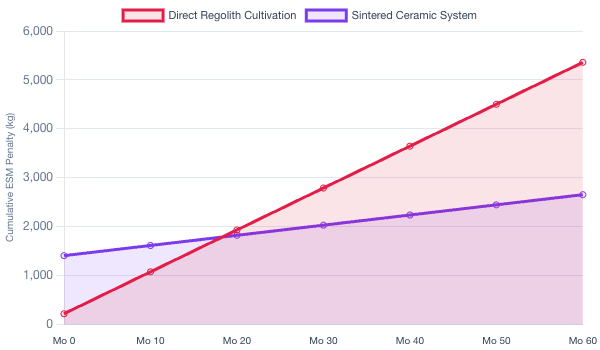
\includegraphics[width=\textwidth]{figures/fig4_esm_lifecycle.png}
        \caption{Cumulative ESM trajectory over 60 months.}
        \label{fig:esm_lifecycle}
    \end{subfigure}
    \hfill
    \begin{subfigure}[b]{0.48\textwidth}
        \centering
        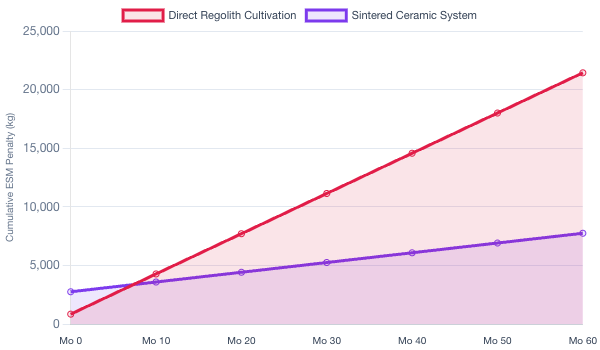
\includegraphics[width=\textwidth]{figures/fig5_mission_economics.png}
        \caption{Crew scaling and mission economics comparison.}
        \label{fig:mission_economics}
    \end{subfigure}
    \caption{\textbf{Equivalent System Mass (ESM) lifecycle economics comparing direct regolith agriculture with sintered ceramic bio-infrastructure.} (\textbf{a}) Cumulative ESM curves for a nominal 6-person habitat over a 60-month horizon, showing operational breakeven between 18 and 22 months. Direct regolith farming starts at lower initial mass ($420\,\mathrm{kg}$) but scales aggressively due to water loss and chemical buffers; sintered infrastructure starts at $1850\,\mathrm{kg}$ but exhibits flat consumable demands. (\textbf{b}) Total lifecycle mass comparison across small (3 crew) and large (12 crew) expeditionary sizes at 60 months.}
    \label{fig:esm_trade_study}
\end{figure}

\begin{table}[t!]
\small
\centering
\caption{\textbf{Systems-level Equivalent System Mass (ESM) lifecycle trade study for a 6-person lunar habitat comparing direct regolith cultivation against sintered ceramic bio-infrastructure.}}
\label{tab:esm_comparison}
\begin{tabularx}{\textwidth}{lXXX}
\toprule
\textbf{Lifecycle Parameter} & \textbf{Direct Regolith Cultivation} & \textbf{Sintered Ceramic System} & \textbf{Systems Advantage Factor} \\
\midrule
Initial Hardware Mass ($M$) & Low ($\sim 420\,\mathrm{kg}$ containment/tools)\cite{ming1989lunar} & High ($\sim 1850\,\mathrm{kg}$ sintering plant)\cite{ming1989lunar,meek1993mechanical} & Direct regolith saves $1430\,\mathrm{kg}$ initial launch mass \\
\addlinespace
Habitat Volume Equivalent ($V \cdot C_V$) & High ($\sim 12.5\,\mathrm{m}^3$ bed margins)\cite{paul2022plants,ming1989lunar,hanford2006baseline} & Compact ($\sim 4.2\,\mathrm{m}^3$ vertical modules)\cite{paul2022plants,ming1989lunar} & Sintering saves $66\%$ pressurized volume \\
\addlinespace
Water Recovery Efficiency ($\eta_{\mathrm{H}_2\mathrm{O}}$) & $78.0\text{--}82.0\%$ (trapped in fines)\cite{paul2022plants,ming1989lunar} & $>98.5\%$ (high-efficiency recycling)\cite{ming1989lunar} & Saves hundreds of kilograms makeup water annually\cite{ming1989lunar,chinnannan2025spirulina} \\
\addlinespace
Consumable Buffers / Chelates & $145\,\mathrm{kg/year}$ ($\mathrm{HNO}_3$, EDTA)\cite{ming1989lunar,schoonen2020hydroxyl} & $<8\,\mathrm{kg/year}$ (minimal chemical drift)\cite{ming1989lunar} & Sintering reduces buffer resupply by $94\%$ \\
\addlinespace
Dust Mitigation Labor ($T \cdot C_T$) & High (continuous cleaning, filter change)\cite{paul2022plants,ming1989lunar} & Negligible (monolithic surfaces)\cite{ming1989lunar} & Eliminates abrasive dust hazards to ECLSS loops\cite{paul2022plants,ming1989lunar,hendrix2024reactivity} \\
\addlinespace
ESM Breakeven Horizon & Favorable only for missions $<18$ months\cite{ming1989lunar} & Cost-optimal for missions $>22$ months\cite{ming1989lunar} & Sintering yields compounding long-term mass savings\cite{ming1989lunar,min2023protection} \\
\bottomrule
\end{tabularx}
\end{table}
